\documentclass[a4paper, 11pt]{report}



\usepackage[utf8]{inputenc} 
\usepackage[T1]{fontenc}
\usepackage{lmodern}
\usepackage{graphicx}
\usepackage[french]{babel}
\usepackage{color}
%\usepackage{fullpage}
\usepackage{array}
\usepackage[tight]{shorttoc}
\usepackage[toc,page]{appendix} 
\usepackage{makeidx} 
\usepackage{titlesec} % pour enlever "chapitre"


\definecolor{gris}{gray}{0.45}

\newcommand{\rouge}[1]{\textcolor{red}{#1}}
\newcommand{\rem}[1]{\textcolor{blue}{\emph{Remarque: \\} #1}}
\newcommand{\exl}[1]{\textcolor{gris}{\emph{Exemple: } #1}}
\newcommand{\exc}[1]{\textcolor{gris}{(\emph{Ex:} #1)}}
\newcommand{\cod}[1]{\textcolor{gris}{\emph{#1}}} 
\newcommand{\att}[1]{\textcolor{red}{\emph{\\ Attention: \\} #1 \\}}

\usepackage{listings}
\definecolor{dkgreen}{rgb}{0,0.6,0}
\definecolor{gray}{rgb}{0.5,0.5,0.5}
\definecolor{mauve}{rgb}{0.58,0,0.82}
\definecolor{red}{rgb}{1,0,0}

\newcommand{\lstconfig}[1]{
	\lstset{
	  language=#1,				      % the language of the code
	  basicstyle=\footnotesize,	      % the size of the fonts that are used for the code
	  numbers=left,				      % where to put the line-numbers
	  numberstyle=\footnotesize,	  % the size of the fonts that are used for the line-numbers
	  stepnumber=1,				      % the step between two line-numbers. If it's 1, each line 
									  % will be numbered
	  numbersep=5pt,				  % how far the line-numbers are from the code
	  backgroundcolor=\color{white},  % choose the background color. You must add \usepackage{color}
	  showspaces=false,			      % show spaces adding particular underscores
	  showstringspaces=false,		  % underline spaces within strings
	  showtabs=false,				  % show tabs within strings adding particular underscores
	  frame=single,				      % adds a frame around the code
	  tabsize=2,					  % sets default tabsize to 2 spaces
	  captionpos=b,				      % sets the caption-position to bottom
	  breaklines=true,				  % sets automatic line breaking
	  breakatwhitespace=false,		  % sets if automatic breaks should only happen at whitespace
	  title=\lstname,	   			  % show the filename of files included with \lstinputlisting;
									  % also try caption instead of title
	  numberstyle=\tiny\color{gray},  % line number style
	  keywordstyle=\color{blue},	  % keyword style
	  commentstyle=\color{dkgreen}\textit,   % comment style
	  stringstyle=\color{mauve}\textbf,	  % string literal style
	}
}

	%\title{\vspace{5cm}Nascar \\ Rapport de projet \\ LO41 \\ \ \\}
	%\date{automne 2012\\ \ \\ \vspace*{3cm}
	%\includegraphics[width=4cm]{logo_utbm.png}
	%}
	%\author{Paul Locatelli - Pierre Rognon \\ \ \\ \ \\ Université de Technologies de Belfort-Montbéliard\\ \ \\}
	
	\titleformat{\chapter}[hang]{\bf\huge}{\thechapter}{2pc}{}     

\begin{document}

\makeatletter
	\def\clap#1{\hbox to 0pt{\hss #1\hss}}%
	\def\ligne#1{%
	\hbox to \hsize{%
	\vbox{\centering #1}}}%
	\def\haut#1#2#3{%
	\hbox to \hsize{%
	\rlap{\vtop{\raggedright #1}}%
	\hss
	\clap{\vtop{\centering #2}}%
	\hss
	\llap{\vtop{\raggedleft #3}}}}%
	\def\bas#1#2#3{%
	\hbox to \hsize{%
	\rlap{\vbox{\raggedright #1}}%
	\hss
	\clap{\vbox{\centering #2}}%
	\hss
	\llap{\vbox{\raggedleft #3}}}}%
	\def\maketitle{%
	\thispagestyle{empty}\vbox to \vsize{%
	\haut{}{\@blurb}{}
	\vfill
	\vspace{1cm}
\begin{flushleft}
	%\usefont{OT1}{ptm}{m}{n}
	\huge \@title
\end{flushleft}
	\par
	\hrule height 4pt
	\par
\begin{flushright}
	%\usefont{OT1}{phv}{m}{n}
	\Large \@author
	\par
\end{flushright}
	\vspace{1cm}
	\vfill
	\vfill

\begin{center}
	
\includegraphics[width=5cm]{logo_UTBM.jpg}
\end{center}

\bas{}{Automne 2012}{}
}%
\cleardoublepage
}
\def\date#1{\def\@date{#1}}
\def\author#1{\def\@author{#1}}
\def\title#1{\def\@title{#1}}
\def\location#1{\def\@location{#1}}
\def\blurb#1{\def\@blurb{#1}}
\date{\today}
\author{}
\title{}

% informations
\location{Belfort}\blurb{}
\makeatother
\title{Projet de résolution d'un tangram}
\author{\small{Adrien \bsc{Berthet} Paul \bsc{Locatelli} et Pierre \bsc{Rognon}}}
\blurb{%
	\textbf{IA41 - Concepts fondamentaux en Intelligence Artificielle et langages dédiés}\\
	Université de Technologie de Belfort-Montbéliard
}% 


	
	\maketitle
	
	\newpage
	
	\shorttoc{Sommaire}{0}
	
	
	\chapter*{Introduction}
	\addcontentsline{toc}{chapter}{Introduction}
	
		Pour ce projet, le sujet abordant le casse-tête du tangram (numéro 6) a été retenu. Le choix de ce sujet s'est fait sur l'intérêt de ce jeu. En effet, s'il apparaît assez aisé de résoudre des modèles tels que le classique "carré" que chacun connaît, d'autres modèles sont beaucoup plus complexes. De plus, c'est un test utilisé dans de nombreux tests afin de déceler d'éventuelles déficiences chez les enfants tels que le WISC (Wechsler Intelligence Scale for Children). C'est donc un problème d'Intelligence Artificielle fondamental qui sera abordé dans ce projet et dont la résolution sera tentée.\\
L'analyse de ce problème constitue une partie prépondérante dans la tentative de résolution du tangram. Environ 6000 configurations différentes sont connues aujourd'hui. De nombreux modèles ont donc dû être envisagés afin de couvrir l'ensemble des cas possibles. Une seconde phase qui s'avère aussi complexe est le choix des différentes représentations informatiques du problème. De nombreux traitements ont été effectués pour mettre à bien cette partie. Quelques exemples qui ont été utilisés comme support durant toute la durée du projet seront présentés afin d'indiquer leur solution. Enfin, la résolution par le logiciel crée sera abordée pour ces exemples. Les limites de ce problème et l'état d'avancement du projet seront indiqués enfin.


	\newpage

	\chapter{Analyse du casse-t\^ete}
	
	Une première analyse du tangram a permis de mettre à jour plusieurs sous-problèmes. Deux problèmes d'ordre mathématique ainsi qu'un problème d'intelligence artificielle pure ont ainsi été isolés. 
	
		\section{Placement de pièce dans un modèle}
		
		Le premier problème à résoudre est le placement d'une pièce dans un modèle. L'objectif de cette méthode est ainsi de renvoyer l'ensemble des positions possibles pour une pièce dans le modèle.\\
		Pour le développement de cette méthode, l'analyse s'est faite sur la base du raisonnement humain. La première approche, la plus simple pour un humain, consiste à tester toutes les positions possibles que peut prendre une pièce.\\
		Si cette approche par\^ait intéressante et rapide à effectuer par un cerveau humain, du point de vue de la programmation et donc de l'intelligence artificielle, cette méthode n'est pas très efficace, puisqu'elle implique de tester toutes les solutions.\\
		Pour une résolution efficace, après étude de différentes possibilités, il est apparu qu'il était préférable de "coller" les pièces à une arête du modèle. Cependant, ce "matching" doit se faire d'une manière intelligente. \\
		Le but est donc de chercher les points communs entre la pièce et le modèle afin de trouver un point ou une arête constituant la base du placement de la pièce. Le premier point commun possible entre la pièce et le modèle est la longueur d'une arête. En effet, les pièces du Tangram ayant chacune des caractéristiques différentes, si une arête du dessin coïncide avec une arête de la pièce, il y a de grandes chances pour que la pièce soit positionnée à cet endroit. 
    
    \begin{center}
    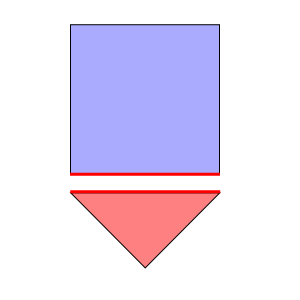
\includegraphics[width=5cm]{place_figure_exacte_match}\\
    \emph{Ici, on peut voir que le triangle a une arête qui coïncide exactement avec une arête du modèle.}\\
    \end{center}

    S'il est évident que cette méthode est efficace dans de nombreux cas, elle a ses limites: il se peut que lors de la résolution du Tangram, une arête du modèle corresponde à plusieurs pièces. Lors de ce type de configurations la première méthode est donc inefficace. 

    \begin{center}
    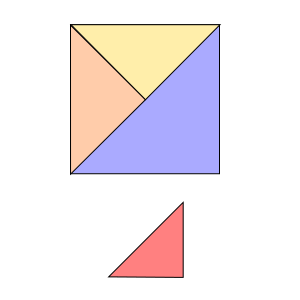
\includegraphics[width=5cm]{place_figure_probleme_exacte_match}\\
    \emph{Un problème peut arriver si plusieurs pièces coïncident avec une arête.}\\
    \end{center}

    Un second point commun, qui va pouvoir résoudre le problème précédent, a été trouvé. Cette seconde caractéristique commune, utile pour la décision de placement de la pièce, est l'utilisation des angles de chaque pièce. Cette méthode n'est utilisée que lorsque la première méthode est inefficace. Il faut alors vérifier si un angle du modèle est égal à l'un des angles de la pièce. 

    \begin{center}
    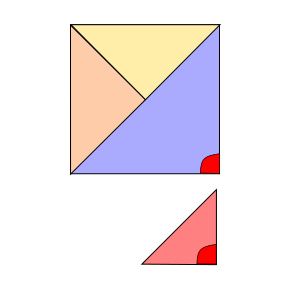
\includegraphics[width=5cm]{place_figure_probleme_angle_match}\\
    \emph{Dans ce cas, on remarque qu'aucune arête ne coïncide. La méthode des angles est donc appliquée et l'on trouve un angle égal.}\\
    \end{center}

    Une fois la base du placement de la pièce trouvée (le point où l'angle correspond entre pièce et modèle), on obtient soit une arête, soit un angle composé de deux arêtes. Il faut ensuite positionner la pièce en fonction de l'arête (ou des arêtes) à l'aide de translation(s) et rotation(s).\\
    Cependant une fois la pièce correctement placée sur le modèle par rapport à la base, un problème important demeure. En effet, selon la rotation et le sens initiale de la pièce, celle-ci peut se trouver à l'inverse de la position voulue. 

    \begin{center}
    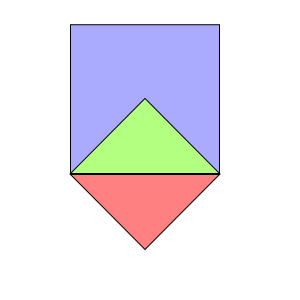
\includegraphics[width=5cm]{place_figure_probleme_symetrie_1}
    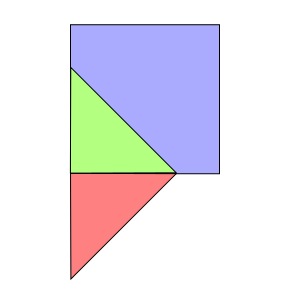
\includegraphics[width=5cm]{place_figure_probleme_symetrie_2}\\
    \emph{Dans les deux figures ci-dessus, la pièce doit être placée sur la surface verte. Cependant, dans certains cas, la méthode indique la surface rouge, dans le mauvais sens, donc.}
    \end{center}

	La validation (ou non) de la position de la pièce est donc le problème le plus important une fois la ou les arêtes communes trouvées entre le modèle et la pièce. Après l'obtention d'une position il faut vérifier si tous les sommets de la pièce font partie de la pièce afin de s'assurer qu'elle n'est pas positionnée dans le mauvais sens ou sur arête qui ne permet pas de placer entièrement la pièce. En effet, il ne faut pas que les pièces se superposent, ni qu'elle soient à l'extérieur du modèle.

    \begin{center}
    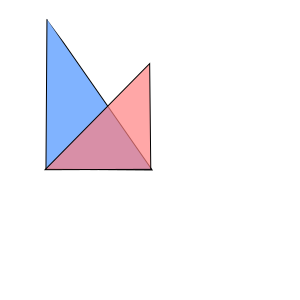
\includegraphics[width=5cm]{place_figure_probleme_point}\\
    \emph{Ici, une arête coïncidente a bien été trouvée mais il n'y a pas la place pour que la pièce se place dans le modèle. Cette pièce peut alors soit être en dehors du modèle initial, soit sur une autre pièce (puisque notre méthode est récursive et que le modèle dans ce cas est une étape).}\\
    \end{center}

    Pour résoudre ce problème, un algorithme existant et assez complexe a été utilisé. Pour chaque sommet de la figure, le nombre d'arêtes ayant un point à la même hauteur que le sommet est compté. Dans le cas où un nombre impair de points de chaque coté de l'arête est trouvé, alors le point est à l'intérieur du modèle. Sinon, il se trouve à l'extérieur.\\
    La source de l'algorithme est disponible à l'adresse suivante : \emph{http://alienryderflex.com/polygon/}\\ 

    Après avoir testé l'ensemble des points de la pièce positionnée et ainsi que l'ensemble des points de son symétrique par rapport à l'arête de la base, l'une des pièces est identifiée comme étant en partie à l'extérieur du modèle.\\ \ \\

    L'algorithme chargé de générer l'ensemble des placements possibles va donc pour une pièce et un modèle donnés, tenter de trouver les positions disponibles. Pour cela, la première méthode va être utilisée puis de la seconde. Dans le deux cas, la validité des résultats trouvés est vérifiée.\\
    Dans le cas où aucun placement n'est possible (c'est à dire si le modèle est trop petit pour accueillir la pièce ou si aucun angle ni aucune arête ne convient), l'algorithme échoue.
	
		\section{Soustraction d'une forme au modèle}
		
		Le second problème mathématique que la résolution exigeait de résoudre est la soustraction d'une forme au modèle. En effet, la solution la plus simple résidait dans le fait de placer une forme dans le modèle pour ensuite renvoyer un nouveau problème et recommencer le casse-t\^ete la forme placée en moins avec le nouveau modèle.
	
	
	\newpage
	
	\chapter{Représentation informatique du problème}
	
	Le passage de la phase d'analyse à la phase "informatique" du pour la résolution du tangram s'avère beaucoup plus complexe que ce qui avait été prévu. Cependant, des représentations précises ont été adoptées. Ces représentations se traduisent par des structures de données fixes qui ont été mises en place afin de mieux coordonner les différents prédicats Prolog.

	    \section{Structures de données}

        La structure majeure qui a dû être mise en place lors de l'implémentation du projet se doit de permettre la définition des pièces du Tangram ainsi que des différentes patterns.\\ \ \\ 
        
        Après avoir envisagé plusieurs solutions il a été décidé de représenter toutes les figures dans un repère orthonormé où chaque point d'une figure est représenté par deux coordonnées X et Y. \\
        En ce qui concerne Prolog, un point est donc représenté par une liste de deux éléments où le premier est la coordonnée en abscisse (X) et le second celle en ordonnée (Y).\\
		Comme en géométrie où une figure est définie par un ensemble de points, en Prolog, la représentation des figures se structure selon une liste de points, ces derniers étant ordonnés de façon à ce que deux points l'un à coté de l'autre dans la liste forment une arête sur la figure. Plus simplement, les points sont placés dans l'ordre. Bien entendu, le couple formé par le premier et le dernier point représente également une arête.\\
		Les pièces sont donc représentées par des listes de points, chacune de ces pièces ayant un point qui est positionné à l'origine du repère. Grâce à cette modélisation, lors du placement des pièces sur un modèle, il suffira de transformer la figure par rotation ou par translation vers sa position.\\
		Les modèles sont un peu plus complexes à modéliser car ils peuvent être divisés en plusieurs parties pour certaines configurations. Aussi, comme il n'est pas possible de prévoir la position des pièces à l'avance, il se peut que le positionnement d'une pièce dans le modèle forme deux nouveaux sous modèles. Il a donc été choisi de modéliser un modèle suivant une liste de figures. 


        \begin{center}
            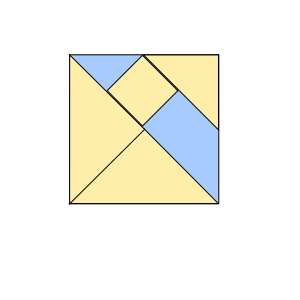
\includegraphics[width=5cm]{representation_sousfigure}\\
            \emph{Dans le cas ci-dessus, on remarque que le placement du carré dans le modèle fait passer celui-ci d'une partie à deux en sortie de l'algorithme de soustraction d'une pièce à un modèle.}
        \end{center}

	
	\chapter{Résultats obtenus}
	
	De nombreux problèmes ayant été rencontrés durant le projet, les résultats obtenus n'indiquent pas une résolution totale de différents modèles. Ceci est d\^u au fait des différentes difficultés apparues sur les algorithmes mathématiques touchant à la géométrie.
	
	
		
	\newpage	
		
	\tableofcontents
		
\end{document}




